\chapter{Descrizione della soluzione}
\label{chp:04-solution}
In questo capitolo verrà approfondito l'aspetto puramente pratico e le fasi che hanno portato alla realizzazione della soluzione; 
inoltre verranno mostrate le applicazioni pratiche degli aspetti teorici enunciati nei capitoli precedenti, unitamente alle difficoltà 
principali incontrate.


Prima di poter costruire il sistema di raccomandandazione proposto in questa tesi, sono state eseguite delle operazioni preliminari
per poter impostare il progetto di Django e la relativa applicazione che implementerà effettivamente la soluzione.
Dalla Figura \ref{fig:str_django_project} è possibile osservare come viene strutturato il progetto, le relative cartelle e file.\\

\begin{figure}
	\centering
	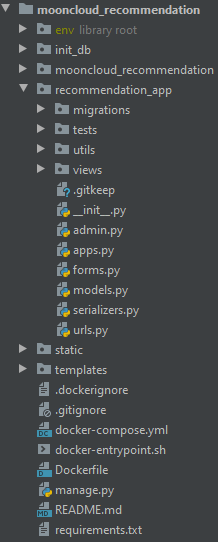
\includegraphics[scale=0.7]{images/str_django_project.png}
	\caption{Struttura dell'applicativo sfruttando il framework proposto da Django}
	\label{fig:str_django_project}
\end{figure}

Il primo passo compiuto e fondamentale è stato quello di disegnare una base di dati da cui partire per la realizzazione degli algoritmi 
proposti.
In generale Moon Cloud possiede una struttura delle Evaluation ad albero, quindi anche di conseguenza anche le tabelle del database 
rispecchiano questa struttura, sulla base delle considerazioni sulle tecniche adottate sono state fatte nei capitoli precendenti.\\
Per implementare un modified pre-order trasversal tree in Django, si è fatto uso del package MPTT, come detto in precendenza, questa
tecnica è usata per memorizzare dati gerarchici in un database, puntando all'efficenza nelle operazioni di recupero dei dati e 
scendendo a compromessi per quanto riguarda le operazioni di inserimento e spostamento dei nodi all'interno della struttura.
Grazie all'usilio di questa utility ai Models 


\begin{figure}
	\centering
	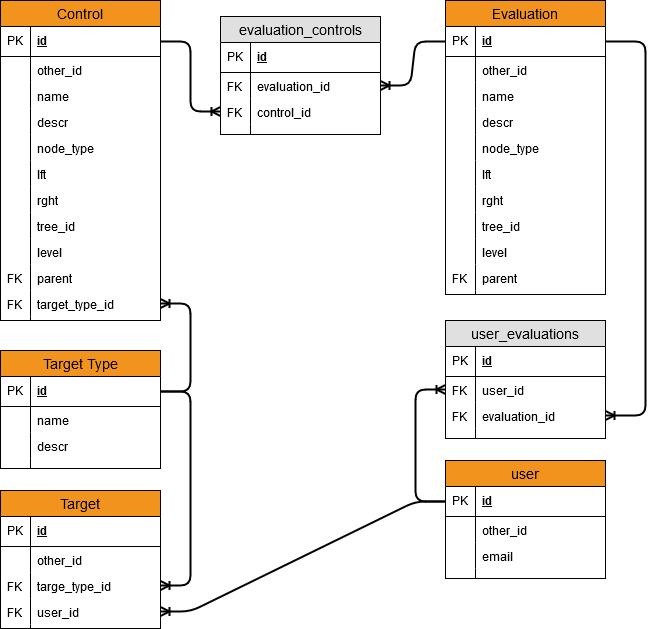
\includegraphics[scale=0.7]{images/MoonCloudRecommendation_ER.png}
	\caption{Struttura del database}
	\label{fig:str_db_project}
\end{figure}

Si è pensato di introdurre una tabella Evaluation, che continene l'insieme di Evaluation che un utente può eseguire per un certo Target,
una tabella Control, che rappresenta l'insieme di controlli che possono comporre un Evaluation, una tabella TargetType, che definisce
i tipi di Target supportati da MoonCloud su cui è possibile effettuare i monitoraggi, la tabella Target, raccoglie quali Target un 
utente ha inserito e possono essere più di uno.

% TASSONOMIE E DATABASE CON I MODELS (package MPTT)
Come annunciato nei capitoli precendenti per procedere alla costruzione di un sistema di raccomandazione bisogna avere a disposizione
una base di dati solida da cui attingere tutte le informazioni; ed è proprio questo il primo passo che è stato seguito, 

% ASPETTI DI DJANGO CHE HO PERSONALIZZATO, COME LE ADMIN PAGE

% URLS e VIEW A SCOPO DIDATTICO

% VIEW PER LE RACCOMANDAZIONI

% VIEW PER MANTERE LA CONSISTENZA COL MIO DATABASE

% IMPLEMENTAZIONE CON DOCKER

